%!TEX program = lualatex

\documentclass{article}

\usepackage{amsmath}
\usepackage{fontspec}
\usepackage[a4paper, margin=2cm]{geometry}
\usepackage{graphicx}
\usepackage[hidelinks]{hyperref}

\newcommand{\DISCIPLINE}{Бази даних}
\newcommand{\STUDENT}{}
\newcommand{\SUBJECT}{Побудова ER-моделі предметної області}
\newcommand{\TEACHER}{}
\newcommand{\TITLE}{Лабораторна робота №1}
\newcommand{\VARIANT}{33}

\begin{document}

\setmainfont{OpenSans}
\setlength{\emergencystretch}{2cm}

\clearpage\begin{titlepage}
	\begin{center}
		\Large
		Міністерство освіти і науки України \\
		Національний технічний університет України \\
		«Київський політехнічний інститут імені Ігоря Сікорського» \\
		[1\baselineskip]
		Факультет інформатики та обчислювальної техніки \\
		Кафедра інформатики та програмної інженерії \\
	\end{center}

	\vfill

	\begin{center}
		\Large
		\textbf{\TITLE} \\
		з дисципліни \textbf{«\DISCIPLINE»} \\
		на тему: «\SUBJECT»
	\end{center}

	\vfill

	\begin{center}
		\large
		\textbf{Виконав} \hfill \noindent \hrulefill \STUDENT \hrulefill \\
		\small (шифр, прізвище, ім'я, по батькові) \\
		[1\baselineskip]
		\large
		\textbf{Перевірив} \hfill \noindent \hrulefill \TEACHER \hrulefill \\
		\small (прізвище, ім'я, по батькові) \\
	\end{center}

	\vfill

	\begin{center}
		\Large
		Київ \the\year{}
	\end{center}
\end{titlepage}


\clearpage\tableofcontents

\clearpage\section{Мета}

Отримання навичок моделювання предметної області та побудови ER-моделі
предметної області (діаграм "Сутність-Зв'язок").

\section{Робота рієлторської компанії}

У рієлторську компанію звертаються клієнти, які бажають продати/купити чи зняти/здати нерухомість
у оренду. Компанія визначає рієлтора, який буде вести справи клієнтів, на підставі поточної
завантаженості працівників. Виділений рієлтор реєструє клієнта, його контактні дані, тип та
адресу нерухомості, вартість та інші характеристики, а також статус (здача в оренду, продаж,
здача в оренду або продаж). Склад і кількість характеристик може змінюватись відповідно до типу
нерухомості. При виникненні запиту на нерухомість рієлтор зв'язується з клієнтами і погоджує
зручний час і дату огляду нерухомості.

У разі згоди потенційного орендаря на оренду чи покупця на покупку нерухомості рієлтор зв'язується
з ним і погоджує дату оформлення договору про оренду чи покупку. Для здійснення угоди рієлтор оформляє
необхідні дозволи, документи, контракти та договори, після чого передає їх у центральний апарат
компанії для кінцевого нотаріального засвідчення. Вартість послуг рієлтора складає або половину
місячної вартості оренди нерухомості у випадку здачі в оренду, або 2\% від суми угоди при продажі нерухомості.

Клієнти можуть публікувати власні оголошення на оренду чи продаж, але вони публікуються тільки після
проходження модерації адміністратором. В кінці кожного місяця формується звіт про надані рієлторські
послуги та загальний прибуток по кожному типу нерухомості. За результатами аналізу звіту центральний
апарат компанії приймає рішення щодо розширення або звуження штату працівників. Пошуком пропозицій
на здачу в оренду чи продаж нерухомості також займається центральний апарат фірми.

\section{Постановка задачі}

\begin{enumerate}
      \item Вивчити основні теоретичні засади проектування баз даних, семантичного моделювання,
            побудови ER-діаграм (моделей "сутність-зв'язок")
      \item Виділити основні множини сутностей, їх атрибути, зв'язки між ними згідно наданого опису
            предметної області. Мінімальна кількість сутностей - 6.
      \item Побудувати ER-модель предметної області.
      \item За бажанням декомпозувати зв'язки "багато-до-багатьох".
\end{enumerate}

\clearpage\section{ER-діаграма}

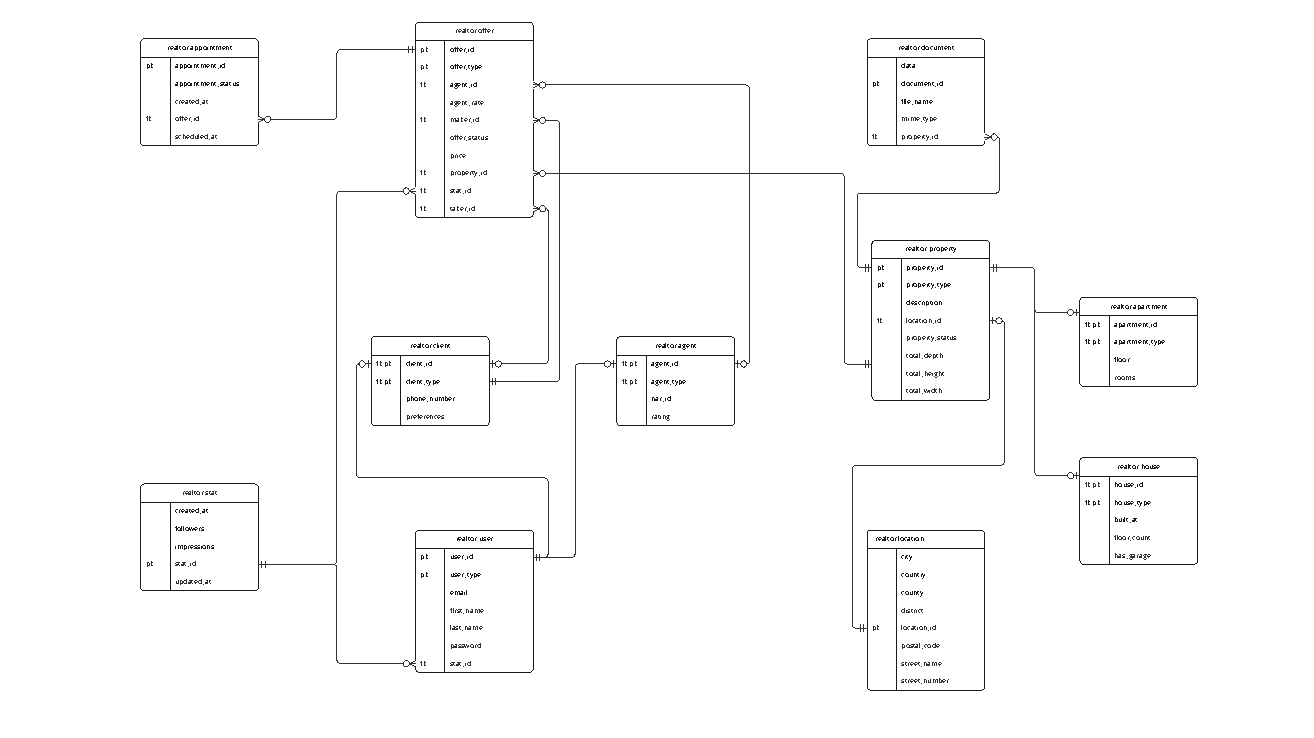
\includegraphics[width=1\linewidth]{../assets/er.pdf}

\section{Зв'язки}

\clearpage\section{Контрольні запитання}

\begin{enumerate}

    \item \textbf{Які кроки включає процес розробки бази даних?}

          \begin{enumerate}
              \item Початкова розробка
                    \begin {enumerate}
              \item Аналіз предметної області
              \item Постановка задачі
              \item Визначення цілей
              \item Визначення сфери дій
          \end{enumerate}

    \item Аналіз концептуальних вимог та інформаційних потреб

          \begin{enumerate}
              \item Аналіз вимог користувачів до бази даних
              \item Виявлення наявних задач по обробці інформації котра повинна бути в базі даних
              \item Виявлення перспективних задач
              \item Документування результатів аналізу
          \end{enumerate}

    \item Реалізація та завантаження БД

          \begin{enumerate}
              \item Встановлення СУБД
              \item Створення БД
              \item Завантаження чи конвертування даних
          \end{enumerate}

    \item Тестування та оцінки БД

          \begin{enumerate}
              \item Тестування БД
              \item Оцінка БД і прикладних програм
          \end{enumerate}
\end{enumerate}

\item \textbf{Що таке предметна область?}

Предметна область – це частина реального світу, дані про яку зберігаються в базі даних.

\item \textbf{Дайте означення моделі предметної області.}

Модель предметної області — шаблон проєктування, який пропонує реалізувати
бізнес-логіку, використовуючи підхід ООП.

\item \textbf{Чим характеризується логічна модель даних?}

Логічна модель - це версія концептуальної моделі для конкретної моделі даних.
Логічне програмування - це процес створення логічної моделі даних на рівні записів
для досліджуваної предметної області. Для реляційних моделей на цьому етапі
фіксується набір і структура таблиць, що представляють сутності, визначаються
ключі і проводиться нормалізація таблиць.

\item \textbf{Дайте означення фізичної моделі даних.}

Фізична модель - є відображенням логічної на об'єкти конкретної СУБД.
Фізичне програмування - це процес створення опису реалізації БД на вторинних
запам'ятовуючих пристроях із вказівкою структур збереження і методів доступу,
використовуваних для організації ефективної обробки даних.

\item \textbf{Для чого використовуються ER-діаграми?}

Діаграма сутностей і зв'язків - це графічне представлення множин сутностей,
їхніх атрибутів та зв'язків. Ці елементи є вершинами графу.

\item \textbf{Назвіть основні складові ER-діаграми?}

Для вказання належності елемента ддо певного виду використовуються:

\begin{enumerate}
    \item прямокутник - для множин сутностей
    \item овал - для атрибутів
    \item ромб - для зв'язків
\end{enumerate}

\item \textbf{Які типи зв'язків використовуються в ER-діаграмах?}

\begin{enumerate}
    \item один до одного
    \item один до багатьох
    \item багато до багатьох
\end{enumerate}

\item \textbf{Як відображаються зв'язки в ER-діаграмах?}

Для розробки баз даних існує декілька типів ER-діаграми:

\begin{enumerate}
    \item Chen's Notation - використовує прямокутники для представлення сутностей і ромби для представлення відносин.
          Для відображення кардинальності використовується буква m, яка позначає багато з одного боку відношення.
          Для позначення одного і тільки одного використовується 1.
    \item Crow's Foot Notation - відносини представлені лініями між квадратами з різними формами,
          або вилками наприкінці, щоб показати кардинальність.
\end{enumerate}

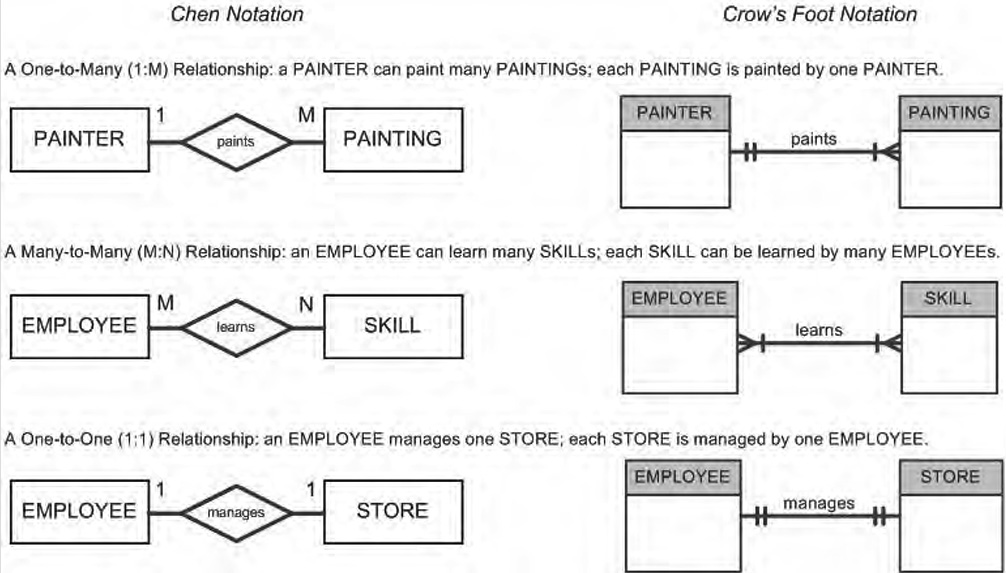
\includegraphics[width=1\linewidth]{../assets/chen-crowsfoot-notation.jpg}

\end{enumerate}


\end{document}
